%---- IMPORTANTE ----
% Esta plantilla está basada en las recomendaciones de la guía "Trabajo fin de Grado: Escribir el TFG", que encontrarás en http://uc3m.libguides.com/TFG/escribir
% contiene recomendaciones de la Biblioteca basadas principalmente en estilos APA e IEEE, pero debes seguir siempre las orientaciones de tu Tutor de TFG y la normativa de TFG para tu titulación.
% Encontrarás un ejemplo de TFG realizado con esta misma plantilla en el archivo "ejemplo_TFG_2017.zip", incluido en la misma carpeta. Consúltalo porque contiene ejemplos útiles para incorporar tablas, figuras, listados de código, bibliografía, etc.


%----------
%	CONFIGURACIÓN DEL DOCUMENTO
%----------

\documentclass[12pt]{report} %fuente a 12pt

% MÁRGENES: 2,5 cm sup. e inf.; 3 cm izdo. y dcho.
\usepackage[
a4paper,
vmargin=2.5cm,
hmargin=3cm
]{geometry}

% INTERLINEADO: Estrecho (6 ptos./interlineado 1,15) o Moderado (6 ptos./interlineado 1,5)
\renewcommand{\baselinestretch}{1.15}
\parskip=6pt

% soporte para generar PDF/A --es importante de cara a su inclusión en e-Archivo porque es el formato óptimo de preservación y a la generación de metadatos, tal y como se describe en http://uc3m.libguides.com/ld.php?content_id=31389625. En la carpeta incluímos el archivo plantilla_tfg_2017.xmpdata en el que puedes incluir los metadatos que se incorporarán al archivo PDF cuando lo compiles. Ese archivo debe llamarse igual que tu archivo .tex
\usepackage[a-1b]{pdfx}

\usepackage{hyperref}
\hypersetup{linktoc=all}

% Expresiones matemáticas
\usepackage{amsmath,amssymb,amsfonts,amsthm}

\usepackage{txfonts} 
\usepackage[T1]{fontenc}
\usepackage[utf8]{inputenc}

\usepackage[spanish, es-tabla]{babel} % información sobre el paquete babel para español http://osl.ugr.es/CTAN/language/spanish/babel/base/spanish.pdf
\usepackage[babel, spanish=spanish]{csquotes}
\AtBeginEnvironment{quote}{\small}

% DEFINICIÓN DE COLORES para portada y listados de código
\usepackage{color}
\definecolor{azulUC3M}{RGB}{0,0,102}
\definecolor{gray97}{gray}{.97}
\definecolor{gray75}{gray}{.75}
\definecolor{gray45}{gray}{.45}

% diseño de PIE DE PÁGINA
\usepackage{fancyhdr}
\pagestyle{fancy}
\fancyhf{}
\renewcommand{\headrulewidth}{0pt}
\rfoot{\thepage}
\fancypagestyle{plain}{\pagestyle{fancy}}

% DISEÑO DE LOS TÍTULOS de las partes del trabajo (capítulos y epígrafes o subcapítulos)
\usepackage{titlesec}
\usepackage{titletoc}
\titleformat{\chapter}[block]
	{\large\bfseries\filcenter}
	{\thechapter.}
	{5pt}
	{\MakeUppercase}
	{}
\titlespacing{\chapter}{0pt}{0pt}{*3}
\titlecontents{chapter}
	[0pt]                                               
	{}
	{\contentsmargin{0pt}\thecontentslabel.\enspace\uppercase}
	{\contentsmargin{0pt}\uppercase}                        
	{\titlerule*[.7pc]{.}\contentspage}                 
  
\titleformat{\section}
	{\bfseries}
	{\thesection.}
	{5pt}
	{}
\titlecontents{section}
	[5pt]                                               
	{}
	{\contentsmargin{0pt}\thecontentslabel.\enspace}
	{\contentsmargin{0pt}}
	{\titlerule*[.7pc]{.}\contentspage}

\titleformat{\subsection}
	{\normalsize\bfseries}
	{\thesubsection.}
	{5pt}
	{}
\titlecontents{subsection}
	[10pt]                                               
	{}
	{\contentsmargin{0pt}                          
		\thecontentslabel.\enspace}
	{\contentsmargin{0pt}}                        
	{\titlerule*[.7pc]{.}\contentspage}  


% DISEÑO DE TABLAS. Puedes elegir entre el estilo para ingeniería o para ciencias sociales y humanidades. Por defecto, está activado el estilo de ingeniería. Si deseas utilizar el otro, comenta las líneas del diseño de ingeniería y descomenta las del diseño de ciencias sociales y humanidades
\usepackage{multirow} % permite combinar celdas 
\usepackage{caption} % para personalizar el título de tablas y figuras
\usepackage{floatrow} % utilizamos este paquete y sus macros \ttabbox y \ffigbox para alinear los nombres de tablas y figuras de acuerdo con el estilo definido. Para su uso ver archivo de ejemplo 
\usepackage{array} % con este paquete podemos definir en la siguiente línea un nuevo tipo de columna para tablas: ancho personalizado y contenido centrado
\newcolumntype{P}[1]{>{\centering\arraybackslash}p{#1}}
\DeclareCaptionFormat{upper}{#1#2\uppercase{#3}\par}

% Diseño de tabla para ingeniería
\captionsetup[table]{
	format=upper,
	name=TABLA,
	justification=centering,
	labelsep=period,
	width=.75\linewidth,
	labelfont=small,
	font=small,
}

%Diseño de tabla para ciencias sociales y humanidades
%\captionsetup[table]{
%	justification=raggedright,
%	labelsep=period,
%	labelfont=small,
%	singlelinecheck=false,
%	font={small,bf}
%}


% DISEÑO DE FIGURAS. Puedes elegir entre el estilo para ingeniería o para ciencias sociales y humanidades. Por defecto, está activado el estilo de ingeniería. Si deseas utilizar el otro, comenta las líneas del diseño de ingeniería y descomenta las del diseño de ciencias sociales y humanidades
\usepackage{graphicx}
\graphicspath{{imagenes/}} %ruta a la carpeta de imágenes

% Diseño de figuras para ingeniería
\captionsetup[figure]{
	format=hang,
	name=Fig.,
	singlelinecheck=off,
	labelsep=period,
	labelfont=small,
	font=small		
}

% Diseño de figuras para ciencias sociales y humanidades
%\captionsetup[figure]{
%	format=hang,
%	name=Figura,
%	singlelinecheck=off,
%	labelsep=period,
%	labelfont=small,
%	font=small		
%}


% NOTAS A PIE DE PÁGINA
\usepackage{chngcntr} %para numeración contínua de las notas al pie
\counterwithout{footnote}{chapter}

% LISTADOS DE CÓDIGO
% soporte y estilo para listados de código. Más información en https://es.wikibooks.org/wiki/Manual_de_LaTeX/Listados_de_código/Listados_con_listings
\usepackage{listings}

% definimos un estilo de listings
\lstdefinestyle{estilo}{ frame=Ltb,
	framerule=0pt,
	aboveskip=0.5cm,
	framextopmargin=3pt,
	framexbottommargin=3pt,
	framexleftmargin=0.4cm,
	framesep=0pt,
	rulesep=.4pt,
	backgroundcolor=\color{gray97},
	rulesepcolor=\color{black},
	%
	basicstyle=\ttfamily\footnotesize,
	keywordstyle=\bfseries,
	stringstyle=\ttfamily,
	showstringspaces = false,
	commentstyle=\color{gray45},     
	%
	numbers=left,
	numbersep=15pt,
	numberstyle=\tiny,
	numberfirstline = false,
	breaklines=true,
	xleftmargin=\parindent
}

\captionsetup[lstlisting]{font=small, labelsep=period}
% fijamos el estilo a utilizar 
\lstset{style=estilo}
\renewcommand{\lstlistingname}{\uppercase{Código}}


%BIBLIOGRAFÍA - PUEDES ELEGIR ENTRE ESTILO IEEE O APA. POR DEFECTO ESTÁ CONFIGURADO IEEE. SI DESEAS USAR APA, COMENTA LAS LÍNEA DE IEEE Y DESCOMENTA LAS DE APA. Si haces cambios en la configuración de la bibliografía y no obtienes los resultados esperados, es recomendable limpiar los archivos auxiliares y volver a compilar en este orden: COMPILAR-BIBLIOGRAFIA-COMPILAR
% Tienes más información sobre cómo generar bibliografía en http://tex.stackexchange.com/questions/154751/biblatex-with-biber-configuring-my-editor-to-avoid-undefined-citations , https://es.sharelatex.com/learn/Bibliography_management_in_LaTeX y en http://www.ctan.org/tex-archive/macros/latex/exptl/biblatex-contrib
% También te recomendamos consultar la guía temática de la Biblioteca sobre citas bibliográficas: http://uc3m.libguides.com/guias_tematicas/citas_bibliograficas/inicio

% CONFIGURACIÓN PARA LA BIBLIOGRAFÍA IEEE
\usepackage[backend=bibtex, style=ieee, isbn=false,sortcites, maxbibnames=5, minbibnames=1]{biblatex} % Configuración para el estilo de citas de IEEE, recomendado para el área de ingeniería. "maxbibnames" indica que a partir de 5 autores trunque la lista el primero (minbibnames) y añada "et al." tal y como se utiliza en el estilo IEEE.

%CONFIGURACIÓN PARA LA BIBLIOGRAFÍA APA
%\usepackage[style=apa, backend=biber, natbib=true, hyperref=true, uniquelist=false, sortcites]{biblatex}
%\DeclareLanguageMapping{spanish}{spanish-apa}

% Añadimos las siguientes indicaciones para mejorar la adaptación de los estilos en español
\DefineBibliographyStrings{spanish}{%
	andothers = {et\addabbrvspace al\adddot}
}
\DefineBibliographyStrings{spanish}{
	url = {\adddot\space[En línea]\adddot\space Disponible en:}
}
\DefineBibliographyStrings{spanish}{
	urlseen = {Acceso:}
}
\DefineBibliographyStrings{spanish}{
	pages = {pp\adddot},
	page = {p.\adddot}
}

\addbibresource{bibliografia/bibliografia.bib} % llama al archivo bibliografia.bib que utilizamos de ejemplo


%-------------
%	DOCUMENTO
%-------------

\begin{document}
\pagenumbering{roman}
	
%----------
%	PORTADA
%----------	
\begin{titlepage}
	\begin{sffamily}
	\color{azulUC3M}
	\begin{center}
		\begin{figure}[H] %incluimos el logotipo de la Universidad
			\makebox[\textwidth][c]{
\includegraphics[width=16cm]{Portada_Logo.png}}
		\end{figure}
		\vspace{2.5cm}
		\begin{Large}
			Grado Ingeniería de Sistemas Audiovisuales\\			
			2018-2019\\
			\vspace{2cm}		
			\textsl{Trabajo Fin de Grado}
			\bigskip
			
		\end{Large}
		 	{\Huge ``Diseño e implementación de un microservicio con Spring''}\\
		 	\vspace*{0.5cm}
	 		\rule{10.5cm}{0.1mm}\\
			\vspace*{0.9cm}
			{\LARGE Jesús Rienda Iáñez}\\ 
			\vspace*{1cm}
		\begin{Large}
			Tutor/es\\
			Carmen Pelaez Moreno\\
			Leganés, 2019\\
		\end{Large}
	\end{center}
	\vfill
	\color{black}
	
\includegraphics[width=4.2cm]{imagenes/creativecommons.png}\\
	\emph{[Incluir en el caso del interés en su publicación en el archivo abierto]}\\
	Esta obra se encuentra sujeta a la licencia Creative Commons \textbf{Reconocimiento - No Comercial - Sin Obra Derivada}
	\end{sffamily}
\end{titlepage}

\newpage %página en blanco o de cortesía
\thispagestyle{empty}
\mbox{}

%----------
%	RESUMEN Y PALABRAS CLAVE
%----------	
\renewcommand\abstractname{\large\bfseries\filcenter\uppercase{Resumen}}
\begin{abstract}
\thispagestyle{plain}
\setcounter{page}{3}
	
	% ESCRIBIR EL RESUMEN AQUÍ
	
	\textbf{Palabras clave:}
	% Escribir las palabras clave aquí
	
	\vfill
\end{abstract}
	\newpage %página en blanco o de cortesía
	\thispagestyle{empty}
	\mbox{}


%----------
%	DEDICATORIA
%----------	
\chapter*{Dedicatoria}

\setcounter{page}{5}
	
	% ESCRIBIR LA DEDICATORIA AQUÍ	
		
	\vfill
	
	\newpage %página en blanco o de cortesía
	\thispagestyle{empty}
	\mbox{}
	

%----------
%	ÍNDICES
%----------	

%--
%Índice general
%-
\tableofcontents
\thispagestyle{fancy}

\newpage %página en blanco o de cortesía
\thispagestyle{empty}
\mbox{}

%--
%Índice de figuras. Si no se incluyen, comenta las líneas siguientes
%-
\listoffigures
\thispagestyle{fancy}

\newpage %página en blanco o de cortesía
\thispagestyle{empty}
\mbox{}

%--
%Índice de tablas. Si no se incluyen, comenta las líneas siguientes
%-
\listoftables
\thispagestyle{fancy}

\newpage %página en blanco o de cortesía
\thispagestyle{empty}
\mbox{}


%----------
%	TRABAJO
%----------	
\clearpage
\pagenumbering{arabic} % numeración con múmeros arábigos para el resto de la publicación	

\chapter{Introducción}

	% COMENZAR A ESCRIBIR EL TRABAJO
	
	\section{Planteamiento del problema}
	Contamos con datos reales sobre listas de reproducción de Spotify en formato json los cuales contienen información de cada lista y las canciones que contiene.
	Por otra parte tenemos datos de usuarios con las canciones que escuchan.
	

		Necesitamos almacenar estos datos en una base de datos para posteriormente consultarla, actualizarla o crear nuevos registros. 
		Podríamos actuar directamente sobre la base de datos con un cliente pero no seria admisible para un usuario final. 
		Por tanto tendremos que crear un programa el cual haga las consultas a la bbdd y devuelva los datos en un formato optimo para mostrarlos por pantalla.
		Para ello Por lo que necesitamos crear un programa que al invocar nos devuelva los datos almacenados con un tratamiento especifico y un formato definido. Necesitamos que sea sencillo y simple para el cliente que va a consumir dicho servicio. 
		Por ejemplo uno de los tratamiento necesarios sería filtrar las listas en función de las canciones que escuche cada usuario, si ha escuchado mas de 3 canciones de una, deberíamos devolverla.
		
		Este programa tendrá que tener una alta disponibilidad y escalarse cuando sea necesario para siempre tener unos tiempos de respuesta bajos. Ya que existe una gran cantidad de personas que van a consumir el programa al mismo tiempo en determinadas franjas horarias.
		
	\section{Solución propuesta}
	Para la solución de nuestro problema vamos a necesitar productos de distintos proveedores, ya que cada pequeña parte del programa la gestiona un software diferente.
	
	Uno de los puntos mas importantes a decidir seria que base de datos usar, en este caso usaremos CosmosDB.
	Como pieza de software que se comunique con la bbdd, trate lso datos y los devuelva crearemos un servicio web mediante la arquitectura de microservicios desarrollado en java con el framework Spring Boot.
	Como protocolo para la transferencia de datos usaremos REST apoyándonos en sus verbos GET, POST, PUT y DELETE.
	
	\section{Justificación de la solución}
	
	La arquitectura de microservicios pretende dividir una aplicación compleja en pequeños servicios que solo realicen una función especifica y se comuniquen entre ellos para formar la aplicación final.
	
	Cada microservico es totalmente independiente de desarrollar frente al conjunto, lo cual nos viene genial ya que nuestra idea es realizar una pequeña aplicación que aceda a una base de datos y en un futuro ampliar a varias aplicaciones o incluso un frontal. Los microservicios nos permiten desarrollar cada una en un lenguaje de programación diferente.
	
	Al no disponer de una maquina donde desplegar la aplicación, es ideal que los microservicios lleven un servidor de despliegue(tomcat) embebido y así desplegar en la nube dentro de un contenedor de aplicaciones(Dockers).
	
	Una vez desplegado en la nube decidimos que la comunicación sería mediante REST ya que es un protocolo simple y muy eficaz para realizar las distintas operaciones(verbos) en base de datos: añadir, recuperar, actualizar y eliminar, esto en REST seria GET, POST, PUT y DELETE.
	
	En cuanto a base de datos hemos elegido PostgreSQL ya que es open source y totalmente compatible con muchos lenguajes de programación, no solo con Java que es el caso de nuestra aplicación, sino que si en un futuro queremos creamos otro microservicio con python sería posible reutilizar la base de datos.
	Ademas también es capaz de responder a gran cantidad peticiones en un mismo instante y no bloquearse, esto es totalmente esencial ya que necesitamos alta disponibilidad.
	 
	\section{Estado del arte}

	En la década de los 60 surgió lo que a día de hoy conocemos como arquitectura de software, esta fue tomando cada vez mas interés hasta que en la década de 1980 se integro totalmente el diseño en el desarrollo de software. 
	
	El Instituto de Ingeniera de Software la define como:
	"La arquitectura de software es una representación del sistema que ayuda a comprender cómo se comportará un programa. 
	
	La arquitectura del software sirve como modelo tanto para el sistema como para el proyecto que lo desarrolla. La arquitectura es la principal portadora de cualidades del sistema, como el rendimiento, la modificabilidad y la seguridad, ninguna de las cuales se puede lograr sin una visión arquitectónica unificadora. La arquitectura es un artefacto para el análisis temprano para asegurar que un enfoque de diseño proporcionará un sistema aceptable. Al construir una arquitectura efectiva, puede identificar los riesgos de diseño y mitigarlos al inicio del proceso de desarrollo."\cite{SoftwareEngineeringInstitute}. 
	
	El sistema se divide en elementos de software también llamados módulos, con propiedades y relaciones existentes entre ellos. Las propiedades de estos elementos pueden ser de dos tipos, internas y externas.
	
	Las \textbf{propiedades internas}  son aquellas que definen el módulo, es decir, el lenguaje en el que está desarrollado y todos los detalles de la implementación de este como pueden ser:
	
	- Entidades dinámicas en tiempo de ejecución como objetos e hilos.
	
	- Entidades lógicas en tiempo de desarrollo como clases y módulos.
	
	- Entidades físicas como nodos o carpetas.	
	
	Las \textbf{propiedades externas} son los contratos que existen entre módulos y que permiten a otros módulos establecer dependencias/conexiones entre ellos. Es de vital importancia que las interfaces que definen los contratos estén bien definidas para la perfecta integración de los elementos.
	
	Es necesario dividir los requerimientos con los que va a contar el sistema en módulos y definir sus propiedades y como se relacionan entre si. Por ejemplo en la figura \ref{fig:microservices} podemos ver la estructura de un sistema basado en microservicios donde aparecen bases de datos, que serian un modulo donde habría que definir sus propiedades, tablas, colecciones de datos, etc; para cada microservicio habría que definir un api en el que se indique la entrada y salida del modulo, el lenguaje en el que se va a desarrollar...; por ultimo tendríamos un módulo de presentación UI(Interfaz de usuario).
	\begin{figure}
		\centering
		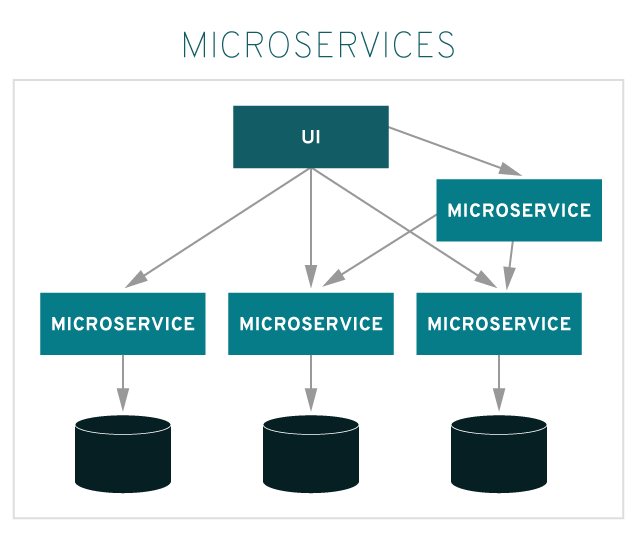
\includegraphics[width=0.7\linewidth]{imagenes/monolithic-vs-microservices}
		\caption{}
		\label{fig:microservices}
	\end{figure}
	
	 En el momento de diseño de una arquitectura existen dos formas de actuar, diseñar una arquitectura desde cero o buscar soluciones ya propuestas a nuestro problema. Si elegimos la segunda opción existen patrones de diseño y frameworks.
	 
	 Los patrones son una forma reutilizable de resolver problemas comunes. Los primeros definidos en arquitectura civil se encuentran en el libro "A pattern language" \cite{PatternLanguage}, en él se describen los patrones con un nombre, de tal manera que con hacer referencia a este, cualquier arquitecto será capaz de entender que solución se está usando sin tener que entrar en detalles. Sin embargo en la arquitectura de software no aparecieron hasta 1994 en un libro que a día de hoy sigue siendo un modelo de referencia\cite{gamma2002patrones}.
	 
	 Los patrones definidos en el libro \cite{gamma2002patrones} se dividen en función del problema a resolver:
	 
	 \begin{itemize}
	 	\item Patrones creacionales: estos son los utilizados para facilitar la creación de nuevos objetos. Los más conocidos son:	 	
	 	\begin{itemize}
	 		\item Abstract Factory: Contiene una interfaz que otorga la creación de objetos relacionados, sin tener que especificar cuáles son las implementaciones concretas.
	 		\item Factory Method: Contiene un método de creación que delega en las subclases la implementación de dicho método.
	 		\item Builder: Con un mismo proceso de construcción nos sirve para crear diferentes representaciones, separando la creación de un objeto complejo de su estructura.
	 		\item Singleton: Solo se permite la creación de una instancia de una clase en nuestro programa y se proporciona un acceso global a el.
	 		\item Prototype: Un objeto se crea a partir de la clonación de otro objeto, es decir se crea basandose en unas "plantillas"
	 	\end{itemize}
 	\item Patrones estructurales: estos nos facilitan la modelización de nuestro software, definiendo la forma en que las clases se relacionan entre si. Los más conocidos son:
 	\begin{itemize}
 		\item Adapter: Mediante un objeto intermedio, se pueden comunicar dos clases con distinta interfaz. 
 		\item Bridge: Se crea un puente entre la abtracción y la implementación, para puedan evolucionar independientemente.
 		\item Composite: Sirve para crear objetos contenidos en un arbol, donde todos los elementos emplean una misma interfaz.
 		\item Decorator: Se añade funcionalidad extra a un objeto (de forma dinámica o estática) sin cambiar su comportamiento.
 		\item Facade: Objeto que crea una interfaz para poder trabajar con otra parte más compleja. Un ejemplo podría ser crear una fachada para trabajar con una librería externa.
 		\item Flyweight: Para ahorrar memoria, gran cantidad de objetos comparten un objeto con las mismas propiedades.
 		\item Proxy: Clase que funciona como interfaz destinada a cualquier otra cosa: conexión a Internet, archivo en disco, etc.
 	\end{itemize}
 	\item Patrones de comportamiento: Se usan para gestionar algoritmos, relaciones y responsabilidades entre objetos. Los más conocidos son: 
 	\begin{itemize}
 		\item Command: Objetos que necesitan para ejecutarse, contener una acción y sus parámetros. 
 		\item Chain of responsibility: Permite pasar solicitudes a lo largo de una cadena de receptores. Al recibir una solicitud, cada controlador decide procesar la solicitud o pasarla al siguiente de la cadena.
 		\item Interpreter: Define una representación y el mecanismo para poder evaluar una gramática. El árbol de sintaxis del lenguaje se modela mediante el patrón \textbf{Composite}.
 		\item Iterator: Nos permite movernos por los elementos de forma secuencial sin necesidad de conocer su implementación.
 		\item Mediator: Objeto que contiene un conjunto de objetos que interactúan y se comunican entre sí.
 		\item Memento: Permite restaurar un objeto a un estado anterior.
 		\item Observer: Objetos que pueden unirse a una serie de eventos que otro objeto va a producir para estar informados cuando esto cambie.
 		\item State: Modifica el comportamiento de un objeto en el tiempo de ejecución.
 		\item Strategy: Selecciona el algoritmo que ejecuta ciertas acciones en tiempo de ejecución.
 		\item Template Method: Nos permite conocer la forma del algoritmo.
 		\item Visitor: Separa el algoritmo de la estructura de datos que se utilizará a la hora de ejecutarlo. Por lo que se pueden añadir nuevas opciones sin tener que ser modificadas.
 	\end{itemize}
	 \end{itemize}
 
 Otra opcion para no diseñar nuestra arquitectura desde cero sería usar frameworks lo cual implica poca implementacion ya que 
	
	Primero surgió la arquitectura orientada objetos mas adelante la orienta a componentes. Pero no fue hasta 1996 cuando se desarrollo por primera vez SOA, arquitectura orientada a servicios. En ella se desarrollaban todos los servicios que tu necesitas conjuntamente y se empaquetan en un war el cual se despliega en un servidor de aplicaciones(tomcat) dentro de una maquina, esto lo podemos ver en la figura \ref{fig:soavsmicroservicios}.
	
	\begin{figure}
		\centering
		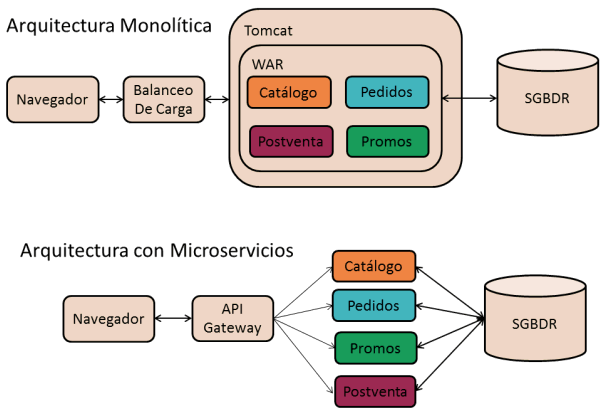
\includegraphics[width=0.7\linewidth]{imagenes/soavsmicroservicios}
		\caption{Arquitectura Monolítica frente Microservicios}
		\label{fig:soavsmicroservicios}
	\end{figure}
	
	Todos los servicios tenían que estar desarrollados con el mismo lenguaje y no  podías asignar mas recursos a uno de ellos sino que se lo asignabas a todo el conjunto, escalando el war en varias maquinas o replicas en la misma. Para ello necesitabas un balanceador de carga antes que determine maquina va a atender tu petición.
	
	Todo esto antes era mas que suficiente para las empresas, pero a día de hoy cuando una aplicación monolítica(SOA) crece mucho es difícil mantener y es complicado añadir nuevas funcionalidades, ya que cada linea modificada implica re-desplegar toda la aplicación, lo que en una empresa grande puede llevar bastante tiempo, ya que en los despliegues normalmente están involucrados varios departamentos de la empresa como seguridad, operaciones, arquitectura y desarrollo, que impide al equipo seguir desarrollando. También es complicado encontrar el origen de algún error en el código.
	
	La necesidad de resolver todos estos problemas desencadeno en la arquitectura de microservicios. La primera vez que se menciono la palabra "microservicios" fue en 2011 en una conferencia sobre computación en la nube donde el Dr. Peter Rogers\cite{breveHistoria} se refirió a ello para describir la arquitectura que estaban usando grandes empresas como Netflix, Facebook, Amazon o PayPal. 
	
	Los microservicios gestionan la complejidad granulando funcionalmente en un conjunto de servicios pequeños e independientes. Con esto se consigue que el equipo de desarrollo sea capaz de desarrollar varias funcionalidades a la vez sin tocar código de otra funcionalidad y desplegar cada modulo por separado tal y como se ve en la figura \ref{fig:soavsmicroservicios} donde cada microservicio esta separado del resto, y puede o no tener una base de datos común.
	
	El cambio mas notable respeto a SOA es que los equipos de desarrollo tienen una mayor responsabilidad, lo que se traduce en una gran facilidad, ya que ellos manejan todo el proceso de desarrollo, desligues en distintos entornos, gestión de contenedores como Kubernetes, etc. Todo esto antes tenían que realizarlo otros departamentos de la empresa con el aumento de tiempos que suponía.
	
	Aunque la arquitectura de microservicios resuelve todos los problemas que presenta SOA y cada vez es mas popular, aun esta en su base de inicio como se menciona en el articulo\cite{Dragoni2017} y aun le queda mucho por mejorar y evolucionar.
	
	Rajest RV en su libro "Spring Microservices"\cite{rv2016spring} nos muestra un gráfico\ref{fig:desarrollomonovsmicro} en el que se ve como es mucho mas rápido y ágil el desarrollo de aplicaciones con microservicios frente a tradicionales. "Los microservicios prometen más agilidad, velocidad de entrega y escala. En comparación con las aplicaciones monolíticas tradicionales."
	
	\begin{figure}
		\centering
		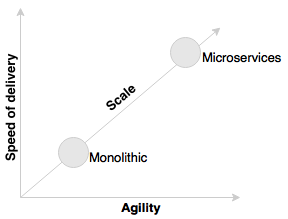
\includegraphics[width=0.7\linewidth]{imagenes/desarrolloMonovsMicro}
		\caption{Eficiencia microservicios frente SOA}
		\label{fig:desarrollomonovsmicro}
	\end{figure}

	En un futuro se deberían solucionar problemas debidos a estar poco restringidos, por ejemplo si cada microservicio lo desarrollas con un lenguaje diferente no esta del todo claro que los protocolos que uses en cada uno de comunicación sean totalmente compatibles. 
	
	En otro tema que tienen que mejorar es en la seguridad, ya que cuando tu descompones una aplicación en cientos de microservicios creas dificultad en la depuración, monitoreo, auditoría y análisis forense de toda la aplicación. Los atacantes podrían aprovechar esta complejidad para atacar.
	
	Lo que si es seguro es que han surgido para quedarse y que cada vez mas gente se esta pasando a ellos.
	


%----------
%	BIBLIOGRAFÍA
%----------	

%\nocite{*} % Si quieres que aparezcan en la bibliografía todos los documentos que la componen (también los que no estén citados en el texto) descomenta está lína

\clearpage
\addcontentsline{toc}{chapter}{Bibliografía}
\setquotestyle[english]{british} % Cambiamos el tipo de cita porque en el estilo IEEE se usan las comillas inglesas.
\printbibliography



%----------
%	ANEXOS
%----------	

% Si tu trabajo incluye anexos, puedes descomentar las siguientes líneas
%\chapter* {Anexo x}
%\pagenumbering{gobble} % Las páginas de los anexos no se numeran



\end{document}